\section{Automatic Diagram Layout with KIELER}

\subsection{Overview}

\eTrice{} provides as a feature the automatic layout of the ROOM diagrams in its graphical editors. This 
helps in improving the pragmatics of the diagrams and frees the user from the burden of manually 
lay-outing the diagrams on the canvas. 

The automatic lay-outing has been provided with the help of the well known KIELER framework, which focuses 
on the pragmatics of model-based system design, which can improve comprehensibility of diagrams, improve 
development and maintenance time, and improve the analysis of dynamic behavior.

This chapter will answer the following questions
\begin{itemize}
\item \hyperref[performLayout]{''How to perform automatic layout in the graphical editors of \eTrice{}?''}
\item \hyperref[layoutOptions]{''What are layout options?''}
\item \hyperref[configureOptions]{''How to configure the layout options to alter the diagram layout as 
desired?''}
\end{itemize}

Moreover, some \hyperref[specialOptions]{''special layout options''} will also be discussed.

\subsection{Performing Automatic Layout}
\label{performLayout}

Automatic layout could be performed in \eTrice{} graphical editors using the command to layout the current 
diagram.

This command is available in

\begin{itemize}
\item The context menu of the diagrams
\item Using the \textit{Ctrl+R L} shortcut.
\end{itemize}

Additionally, an entry in the context menu allows to layout only a selected part of the diagram.

\subsection{Layout Options}
\label{layoutOptions}

A layout option is a customization point for the layout algorithms, with a specific data type and 
optionally a default value, used to affect how the active layout algorithm computes concrete coordinates 
for the graph elements.

User-configurable layout options for a particular diagram object can be viewed and configured through the 
Layout View.The Layout View can be opened from the context menu of a selected diagram object by clicking 
the \textit{Show Layout View} entry. 

On opening the layout view, and selecting any layout option, a description of the layout option is 
available in the footer of eclipse SDK. This is shown in figure \ref{fig:layout_options}.

\begin{figure}
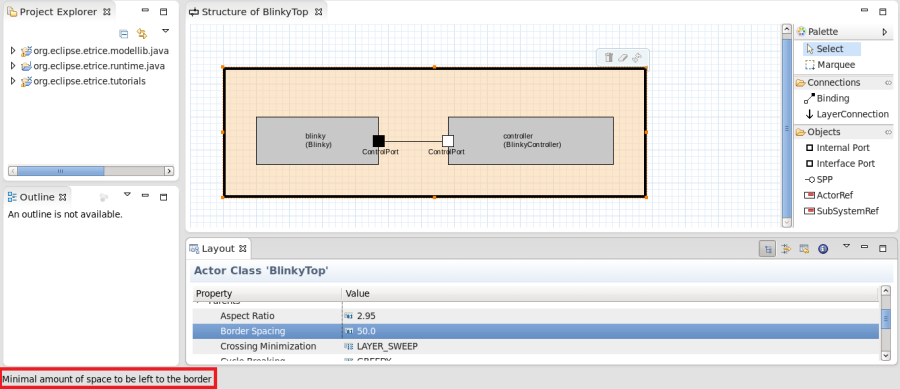
\includegraphics[width=0.8\textwidth]{images/043-LayoutOptionDescription.png}
\caption{Layout options}
\label{fig:layout_options}
\end{figure}

\subsection{Configuring Layout Options}
\label{configureOptions}

The values of the layout options for a particular diagram object (in the visible diagram) can be changed 
using the Layout View of that diagram object. The initial values are the predefined \emph{default} values. 
These defaults can be changed using the context menu in Layout View as well as the Layout preference pages 
provided by \eTrice{}.

\subsubsection{The Layout View}
\label{layoutView}

\begin{figure}
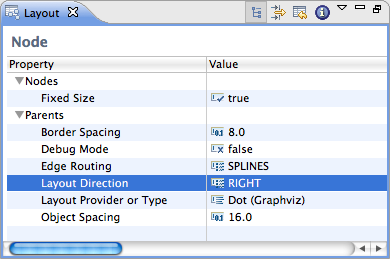
\includegraphics[width=0.5\textwidth]{images/043-LayoutView.png}
\caption{Layout view}
\label{fig:layout_view}
\end{figure}

The Layout view (figure \ref{fig:layout_view}) allows flexible customization of layout options for the selected objects in the \eTrice{} 
diagram. If no object is selected, the view shows the options for the top-level container of the diagram. 
Options are stored persistently in diagram file (\emph{.structure file / }.behavior file) of the \eTrice{} 
diagram, so that they are still available after the next Eclipse restart. Of course this requires the 
diagram to be saved after an option was changed.

The options are grouped according to the function of the selected objects. The group Nodes (respectively 
Edges, Ports, or Labels) contains options related to the object itself, such as its size or priority, 
while the group Parents contains options for the elements contained in the selected objects, such as the 
applied layout algorithm or the spacing between elements. Which layout options are displayed depends on 
the types of selected objects and the active layout algorithm, since each algorithm supports only a subset 
of the available options. Furthermore, some options are only visible if the \textit{Show Advanced 
Properties} button in the view toolbar is activated. The group types can be hidden using the Show 
Categories button.

An option can be changed by selecting or entering a new value in the corresponding cell of the Value column.

The most important option is Layout Algorithm, which is used to determine the layout algorithm for the 
contents of the selected element. Here either a specific layout algorithm or a layout type can be chosen; 
in the latter case, the most suitable layout algorithm of the given type is taken. By changing the active 
layout algorithm, the content of the layout view is updated to display only those options that are 
supported by the new layout algorithm.

Selecting \textit{Restore Default Value} in the context menu or the view toolbar (figure \ref{fig:layout_context_menu})
removes any value for the 
currently selected option that is stored in the current model file, thus resetting the option to its 
default value. The view menu has an entry Remove all Layout Options which resets all options of the 
current model by removing persistent data in the model file.

\begin{figure}
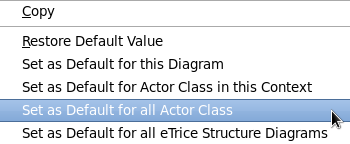
\includegraphics[width=0.4\textwidth]{images/043-ContextMenu.png}
\caption{Layout in context menu}
\label{fig:layout_context_menu}
\end{figure}

The context menu for a specific layout option has different alternatives to set the currently active value 
as \emph{default} value:

\begin{itemize}
\item \emph{Set as Default for this Diagram}: Changes the open diagram file so that the same value is 
applied to all similar objects (edit parts) of that diagram.

\item \emph{Set as Default for ... in this Context}: Applies the value to all similar objects that are 
displayed with the any of the \eTrice{} editors (the option is linked to the edit part class of the selected 
object).

\item \emph{Set as Default for all ...}: Links the option value with the domain model element or the 
diagram type of the selected object (see the context menu depicted above).
\end{itemize}

These four alternatives have different priorities: if present, the default value for the current diagram 
is taken first, then the default value for the edit part is checked, then the default value for the domain 
model element, and then the default value for the diagram type.

Tips:
\begin{itemize}
\item The information button of the view toolbar can be used to display some useful details on the current 
selection, such as the edit part and domain model classes.
\item Default values for layout options can most easily be manipulated based on the \eTrice{} domain model 
elements.
\end{itemize}

\subsubsection{Preference Page}
\label{preferencePage}

The user-defined \emph{default} values for layout options can also be set using the preference pages provided 
in \eTrice{}. Three preference pages have been provided for this purpose
\begin{itemize}
\item \textit{Layout}: for general preferences regarding layout
\item \textit{Behavior}: for setting default values of layout options for \eTrice{} behavior diagrams
\item \textit{Structure}: for setting default values of layout options for \eTrice{} structure diagrams
\end{itemize}

These preference pages can be accessed via \textit{Windows > Preferences > \eTrice{} > Layout}.

Note that the contents of these preference pages are in sync with the \textit{KIELER > Layout} preference 
page provided by the KIELER. Relevant entries in the \textit{KIELER > Layout} page are shown in the above 
preference pages.

\myparagraph{\textit{Layout} Preference Page}

The \textit{Layout} preference page is meant to configure general options regarding the layout. 

If \textit{Set routing style of all edges to oblique} is active, all routing styles and smoothness 
settings of edges are removed when automatic layout is performed. Since most layouters compute the routing 
of edges as part of their algorithm, these styles usually do not yield the expected results.

\myparagraph{\textit{Behavior} and \textit{Structure} Preference Page}


The \textit{Behavior} and \textit{Structure} sub-preference pages help in setting up the default values of 
layout options in behavior and structure diagrams respectively.

The \textit{Default Layout Option Values} table is used to manage the default setting for layout options, 
which can also be modified with the context menu of the layout view (see above). All user-defined settings 
are displayed here, and the buttons on the right of the table serve to create, edit, and remove entries. 
The Type column shows the type of element the option is linked with: either edit part, model element, or 
diagram type. The Element column shows the class name for options that relate to edit parts or domain 
model elements, and the diagram type name for options that relate to diagram types. Option is the name of 
the layout option, and Value is the currently set value of the option.

Creating a new entry requires the selection of the type of related element (figure \ref{fig_layout_preference_page})
and entering its class name or 
identifier. Class names of edit parts can be explored using the information button of the layout view, 
while the class names for the domain model elements and the diagram type identifiers for the diagram types 
can be selected with the Browse button. After that, a layout option has to be selected from the list using 
the corresponding Browse button. Hitting OK creates an entry, and its value can then be set using the Edit 
button.

\begin{figure}
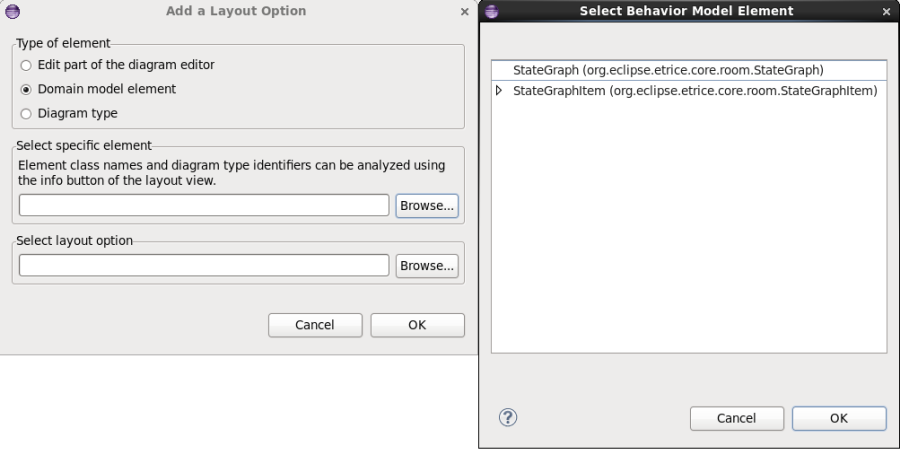
\includegraphics[width=0.8\textwidth]{images/043-PreferencePage.png}
\caption{Layout preference page}
\label{fig_layout_preference_page}
\end{figure}

Note that the \textit{Behavior} preference page will show only those entries which hold for the behavior 
diagrams. Moreover, it will allow setting default values of layout options for only those domain model 
elements and diagram types which could be present in the behavior editor diagrams. Similar thing holds for 
the \textit{Structure} preference page.

\subsection{Special Layout Options}
\label{specialOptions}

While most layout options are used to affect how the active layout algorithm computes concrete coordinates 
for the graph elements, there are some layout options that have a special role.

\subsubsection{Layout Algorithm}

The option with identifier de.cau.cs.kieler.algorithm specifies which layout algorithm to use for the 
content of a composite node. The value can be either the identifier of a layout algorithm or the 
identifier of a layout type. In the latter case the algorithm with highest priority of that type is applied.

For the purpose of automatic diagram layout in \eTrice{}, we use the \textit{Layered} algorithms which are 
meant for lay-outing hierarchical diagrams and are best suited for behavior and structure diagrams in 
\eTrice{}. For the behavior diagrams we have used the \textit{Graphviz Dot} algorithm whereas for the 
structure diagrams we have used the \textit{KLay Layered} algorithm. Though the layout algorithm being 
used for performing layout can be changed at ones own will, it is recommended to use the defaults.  

\subsubsection{Diagram Type}

Diagram types are used to classify graphical diagrams for setting default layout option values for a set 
of similar diagrams. The diagram type of an element is specified with the layout option 
\texttt{de.cau.cs.kieler.diagramType}. Thus, these help in 

The following diagram types have been defined and used in \eTrice{}:
\begin{itemize}
\item \textit{General} - This type is automatically assigned to all diagrams for which no specific type is 
declared. (Predefined in KIELER)
\item \textit{\eTrice{} Behavior Diagrams} - This type has been assigned to the diagram objects in \eTrice{} 
Behavior Diagrams. 
\item \textit{\eTrice{} Structure Diagrams} - This type has been assigned to the diagram objects in \eTrice{} 
Structure Diagrams.
\end{itemize}
Note that not all diagrams objects in the behavior and structure diagrams are assigned the last two 
diagram types. Only the top-level container and the visible bounding box has been assigned these diagram 
types in respective editors.

\subsection{Further References}

Most parts of the above documentation have been taken from the "KIML wiki"
(\url{http://rtsys.informatik.uni-kiel.de/confluence/pages/viewpage.action?pageId=328078}
and have been 
modified for automatic layout in \eTrice{}. A more detailed description about the layout algorithms, 
predefined diagram types and the internal structure of KIELER Infrastructure for Meta-Layout (KIML) can be 
found there.
